\section{Estudio de la API de Spotify}

La API de Spotify es el núcleo del proyecto, ya que proporciona acceso a los datos necesarios para generar las estadísticas y visualizaciones que constituyen el objetivo principal de este trabajo. Este capítulo detalla el análisis realizado sobre la API, explorando sus capacidades, limitaciones y los recursos que ofrece para su integración.

\subsection{Descripción General}

La API de Spotify es una interfaz que permite a las aplicaciones externas interactuar con la plataforma de manera programática. Su propósito principal es proporcionar acceso estructurado a los datos, permitiendo a los desarrolladores integrar funcionalidades avanzadas en sus propias aplicaciones. A través de esta API, es posible obtener información sobre las canciones, artistas, álbumes, listas de reproducción y \textbf{datos personalizados del usuario}, como sus preferencias musicales o sus hábitos de escucha. Gracias a estos últimos, es posible ofrecer una experiencia personalizada para cada usuario.

Entre las características técnicas más destacadas se encuentran:

\begin{itemize}
    \item \textbf{Tipo de API}: RESTful.
    \item \textbf{Protocolo}: HTTPS.
    \item \textbf{Métodos soportados}: \texttt{GET}, \texttt{POST}, \texttt{PUT} y \texttt{DELETE}.
    \item \textbf{Formato de respuesta}: JSON
    \item \textbf{Seguridad}: Acceso protegido mediante OAuth 2.0.
\end{itemize}

Gracias a estas características, la API de Spotify facilita la manipulación de datos gracias a las respuestas en formato JSON, al tiempo que garantiza la seguridad y privacidad del usuario mediante el uso del protocolo OAuth 2.0. Estas cualidades la convierten en una herramienta versátil y segura, capaz de adaptarse a una amplia variedad de proyectos.

\subsection{Autenticación y Autorización}

Antes de avanzar, es importante entender que en este proceso hay dos conceptos clave: \textbf{autenticación} y \textbf{autorización}. Aunque están relacionados, existen ciertas diferencias importantes:

\begin{itemize}
    \item \textbf{Autenticación}: Es el paso en el que se \underline{verifica la identidad} del usuario. En este caso, ocurre cuando el usuario inicia sesión en Spotify para confirmar que es quien dice ser. Este proceso es transparente para el desarrollador ya que Spotify, mediante OAuth 2.0, se encarga de gestionarlo.
    \item \textbf{Autorización}: Es el paso en el que el usuario \underline{concede permisos} para que la aplicación acceda a ciertos recursos de su cuenta. Este proceso es clave, ya que sin estos permisos, la aplicación no podría acceder a los datos necesarios para ofrecer sus funcionalidades.
\end{itemize}

Una vez que la aplicación obtiene la autorización, Spotify permite el acceso a los datos solicitados de forma controlada. Un concepto fundamental en esta etapa son los \textbf{scopes}, que determinan exactamente qué datos y funcionalidades están disponibles para la aplicación.

\subsubsection*{Scopes: Controlando el Acceso a los Recursos} \label{subsubsec:scopes}

Los scopes (alcances) permiten a los usuarios tener la tranquilidad de que únicamente compartirán la información que han autorizado explícitamente. Cuando un programador configura el flujo de autorización, debe especificar los scopes necesarios (de un total de 24) para que la aplicación pueda acceder a los recursos protegidos. En función de los scopes solicitados, Spotify mostrará al usuario una pantalla indicando qué permisos específicos se están requiriendo (figura \ref{fig:auth_popup}). El usuario puede entonces aceptar o rechazar estos permisos.

\begin{figure}[H]
    \centering
    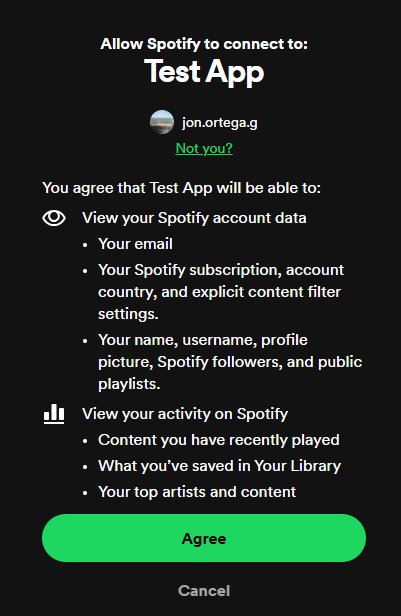
\includegraphics[width=0.3\textwidth]{./figures/auth_popup.png}
    \caption{Pantalla de autorización de scopes en Spotify.}
    \label{fig:auth_popup}
\end{figure}

Una vez que la aplicación obtiene la autorización, el siguiente paso es conseguir el \texttt{access\_token}, necesario para acceder a los recursos autorizados. Un concepto clave para entender cómo se realiza este proceso es el \textbf{authorization flow}, que define las interacciones entre la aplicación, el usuario y Spotify.

\subsubsection*{OAuth Flows: Elegir el Camino Adecuado}

En el marco de OAuth 2.0, el término \textbf{flow} (flujo) se refiere a los diferentes procesos diseñados para obtener un \texttt{access\_token}, dependiendo de las necesidades y características de la aplicación. Estos flujos existen para cubrir una variedad de escenarios, desde aplicaciones web con servidores backend hasta aplicaciones móviles o servicios que no requieren acceso a datos del usuario.

OAuth 2.0 define seis tipos principales de flows, sin embargo, Spotify implementa solo cuatro de ellos (tabla \ref{tab:oauth_spotify_flows}):

\begin{table}[H]
    \centering
    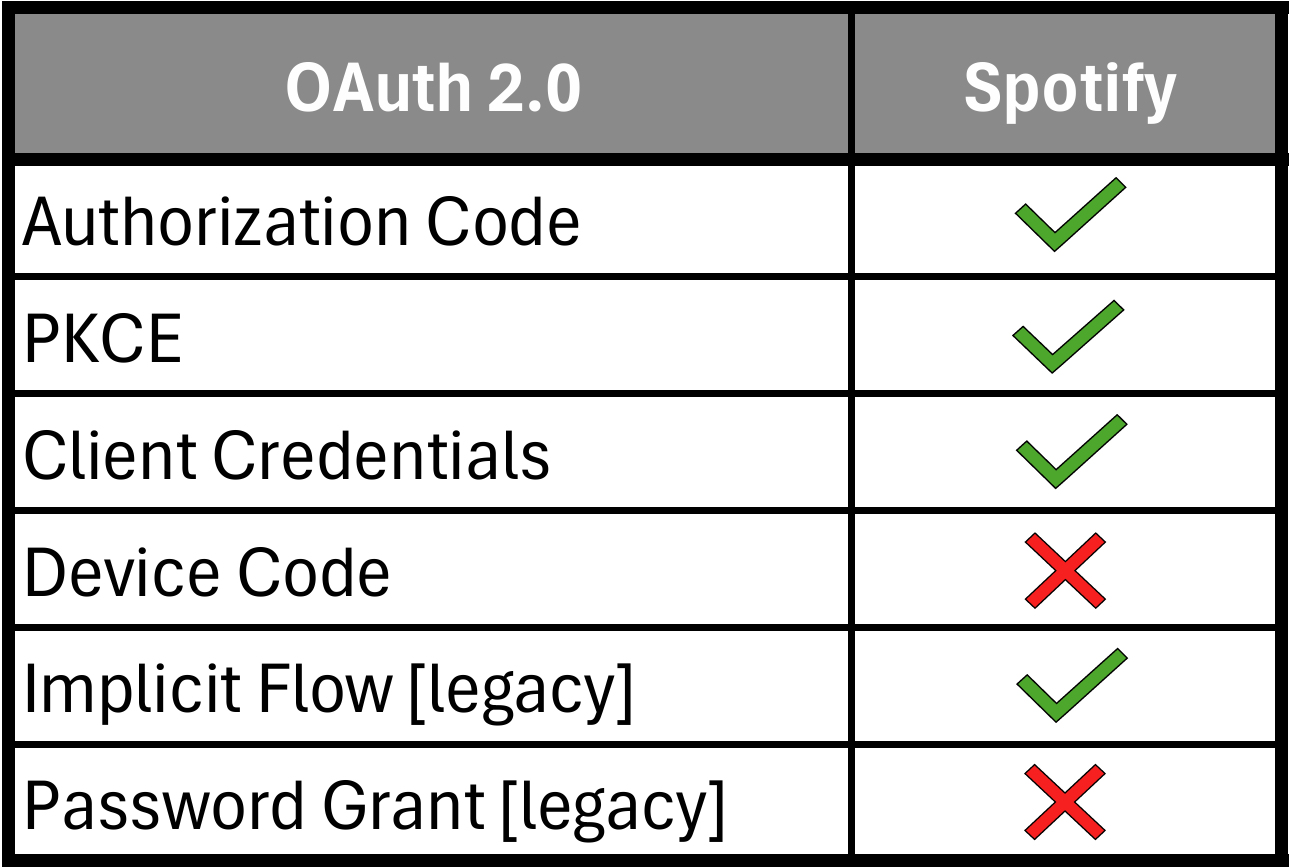
\includegraphics[width=0.5\textwidth]{figures/oauth_vs_spotify_flows.png}
    \caption{Authorization flows definidos por OAuth 2.0 y cuáles implementa Spotify.}
    \label{tab:oauth_spotify_flows}
\end{table}

Cada uno de estos flujos está diseñado para un escenario específico de uso, por lo que, para poder tomar una buena elección, analizaremos las situaciones en las que cada uno resulta más adecuado:

\begin{itemize}
    \item \textbf{Authorization Code Flow}: Ideal para aplicaciones web que cuentan \underline{con un backend} \underline{seguro} donde almacenar el \texttt{client\_secret}. Proporciona tanto un \texttt{access\_token} como un \texttt{refresh\_token}, lo que permite mantener el acceso sin requerir que el usuario se autentique nuevamente. Es el flujo recomendado para aplicaciones con servidores backend que necesitan acceso a datos específicos del usuario.

    \item \textbf{Authorization Code Flow con PKCE}: Es una extensión del anterior, diseñado para \underline{escenarios donde no es seguro almacenar el \texttt{client\_secret}}, como en aplicaciones móviles o \textit{Single Page Applications} (SPA). Añade una capa de seguridad utilizando un \texttt{code\_verifier} y un \texttt{code\_challenge} para evitar que el código de autorización sea interceptado y utilizado de manera malintencionada.

    \item \textbf{Client Credentials Flow}: Adecuado para aplicaciones backend o \underline{servicios que no} \underline{requieren acceso a datos específicos del usuario}, sino que interactúan con recursos de Spotify de manera general. No incluye un proceso de autorización por parte del usuario y no proporciona datos personales.

    \item \textbf{Implicit Grant Flow}: \underline{En desuso debido a limitaciones de seguridad}. Fue diseñado para aplicaciones cliente que no tienen un backend, pero carece de soporte para \texttt{refresh\_tokens} y expone el \texttt{access\_token} en la URL, lo que lo hace menos seguro.
\end{itemize}

De los cuatro flujos de autorización implementados por Spotify, este proyecto utilizará el \textbf{Authorization Code Flow} (sin PKCE). Esta elección se debe a que la aplicación cuenta con un backend seguro implementado con \textit{Route Handlers} de Next.js, lo que permite almacenar de forma segura el \texttt{client\_secret}. Además, este flujo proporciona tanto un \texttt{access\_token} como un \texttt{refresh\_token}, lo que asegura un acceso continuo a los datos del usuario sin necesidad de repetir el proceso de autenticación. Dado que es el flujo recomendado por Spotify para aplicaciones web que necesitan acceder a datos específicos del usuario, garantiza un balance óptimo entre seguridad, funcionalidad y cumplimiento de estándares.

\subsection{Principales Endpoints Relevantes para el Proyecto}

Para facilitar la comprensión de los endpoints utilizados en este proyecto, se ha diseñado un sistema visual que resume la información clave de cada uno, evitando la sobrecarga de texto y permitiendo al lector identificar rápidamente los elementos esenciales.

Cada endpoint se presenta como una interacción entre la solicitud (\textit{request}) y la respuesta (\textit{response}). A la izquierda, la \textit{request} incluye el método HTTP (\texttt{GET}, \texttt{POST}, \texttt{PUT}, \texttt{DELETE}), la URL de la petición y los parámetros requeridos, que pueden estar en la URL (para métodos \texttt{GET}) o en el cuerpo de la solicitud (\textit{body}, para métodos como \texttt{POST} o \texttt{PUT}). Si existen parámetros en los \textit{headers}, se mostrarán sobre los parámetros del \textit{body}/URL. A la derecha se encuentra la \textit{response}, con los campos principales que estarán presentes en el JSON devuelto por la API de Spotify, si la solicitud se procesa correctamente.

En la figura \ref{fig:plantilla_endpoints} se muestra una plantilla genérica que sirve como referencia para entender este sistema visual, que se rellenará con la información específica de cada endpoint en las siguientes secciones.

\begin{figure}[H]
    \centering
    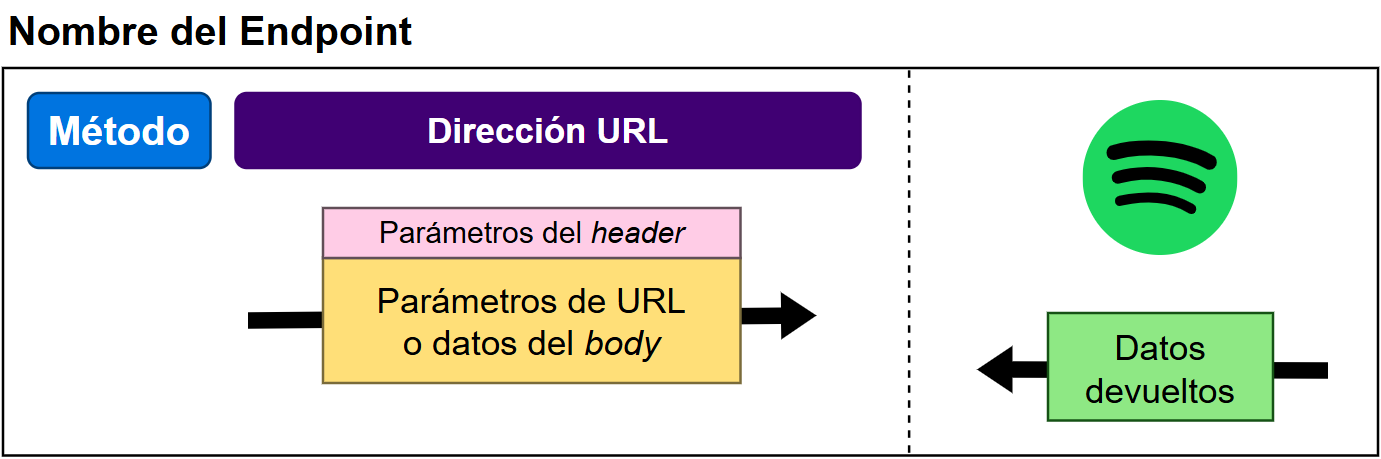
\includegraphics[width=0.95\textwidth]{figures/endpoints/plantilla_endpoints.png}
    \caption{Plantilla visual para representar los endpoints.}
    \label{fig:plantilla_endpoints}
\end{figure}

\subsubsection{Endpoints de Autenticación}

La interacción con Spotify comienza con un endpoint dedicado al proceso de autorización: \textbf{Request User Authorization} (figura \ref{fig:req_usr_auth}). Este endpoint genera la pantalla de autorización que se le muestra al usuario y, en el caso de que acepte, se le redirige a la \texttt{redirect\_uri} indicada en la \textit{request}. En esta URI siempre se suele implementar la llamada al segundo endpoint llamado \textbf{Request Access Token} (figura \ref{fig:req_access_token}), necesario para finalizar el proceso de autorización. Este permite intercambiar el \texttt{code} obtenido en el paso anterior por un \texttt{access\_token}, el cual es requerido para realizar cualquier otra solicitud posterior a la API.

\begin{figure}[H]
    \centering
    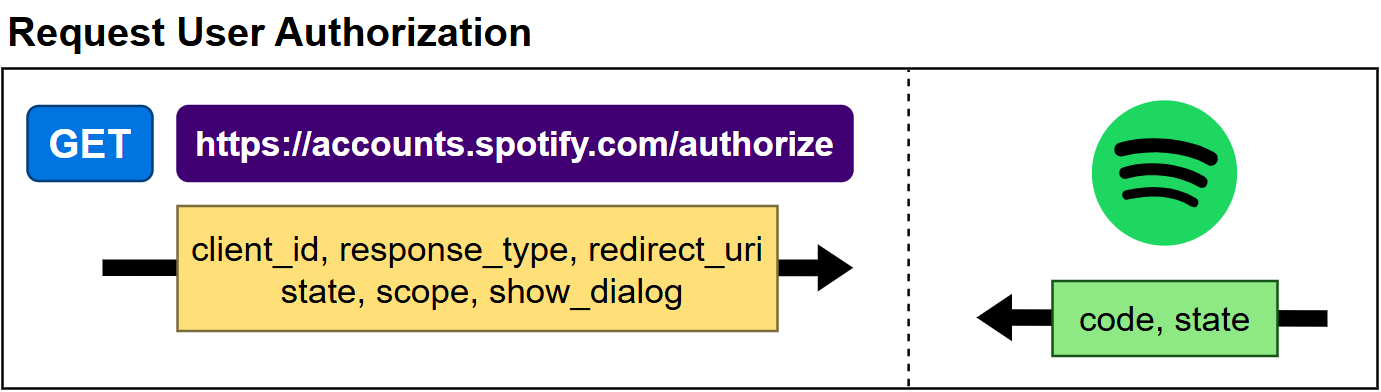
\includegraphics[width=\textwidth]{figures/endpoints/request_user_auth.png}
    \caption{Endpoint de \textit{Request User Authorization}.}
    \label{fig:req_usr_auth}
\end{figure}

\begin{itemize}
    \item \textbf{Parámetros del Request}
          \begin{itemize}
              \item \texttt{client\_id}: El ID de cliente generado al registrar la aplicación.
              \item \texttt{response\_type}: Se establece en \texttt{``code''}, indicando que se solicita un código de autorización.
              \item \texttt{redirect\_uri}: URI a la que se redirige al usuario después de aceptar o rechazar los permisos. Debe coincidir exactamente con uno de los valores configurados al registrar la aplicación.
              \item \texttt{state}: Parámetro utilizado para proteger contra ataques como \textit{cross-site request forgery} (CSRF). Su valor debe ser validado al recibir la respuesta.
              \item \texttt{scope}: Lista de scopes separados por espacios, indicando los permisos requeridos por la aplicación. Si no se especifican, solo se concederá acceso a información pública.
              \item \texttt{show\_dialog}: Determina si se fuerza al usuario a aprobar nuevamente la aplicación, incluso si ya lo hizo previamente. Si se establece en \texttt{true}, el usuario verá el diálogo de autorización; de lo contrario, será redirigido automáticamente.
          \end{itemize}
    \item \textbf{Campos del Response}
          \begin{itemize}
              \item \texttt{code}: Código de autorización que puede intercambiarse posteriormente por un \texttt{access\_token}.
              \item \texttt{state}: El valor del parámetro \texttt{state} enviado originalmente en la solicitud. Su valor debe ser comparado para garantizar la validez de la respuesta.
          \end{itemize}
\end{itemize}

\begin{figure}[H]
    \centering
    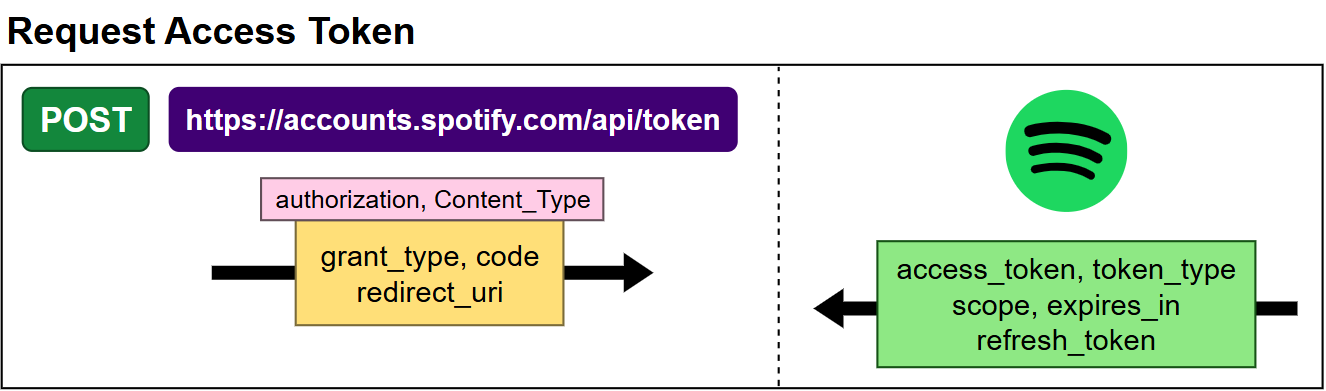
\includegraphics[width=\textwidth]{figures/endpoints/request_access_token.png}
    \caption{Endpoint de \textit{Request Access Token}.}
    \label{fig:req_access_token}
\end{figure}

\begin{itemize}
    \item \textbf{Parámetros del Request}
          \begin{itemize}
              \item \textbf{Body}
                    \begin{itemize}
                        \item \texttt{grant\_type}: Este campo debe contener el valor \texttt{``authorization\_code''}.
                        \item \texttt{code}: El código de autorización devuelto de la solicitud previa.
                        \item \texttt{redirect\_uri}: Este parámetro se utiliza únicamente para validación (no se realiza una redirección real). El valor debe coincidir exactamente con el valor de \texttt{redirect\_uri} utilizado al solicitar el código de autorización.
                    \end{itemize}
              \item \textbf{Headers}
                    \begin{itemize}
                        \item \texttt{Authorization}: Cadena codificada en Base64 con el siguiente formato: \texttt{Basic <base64 encoded client\_id:client\_secret>}.
                        \item \texttt{Content-Type}: Establecido en \texttt{``application/x-www-form-urlencoded''}.
                    \end{itemize}
          \end{itemize}
    \item \textbf{Campos del Response}
          \begin{itemize}
              \item \texttt{access\_token}: Token de acceso que permite hacer las posteriores llamadas a la API.
              \item \texttt{token\_type}: Indica cómo se puede usar el token de acceso; siempre tiene el valor \texttt{``Bearer''}.
              \item \texttt{scope}: Lista de copes separados por espacios que han sido concedidos para este \texttt{access\_token}.
              \item \texttt{expires\_in}: Periodo de tiempo (en segundos) durante el cual el token de acceso es válido. Siempre es de 1 hora.
              \item \texttt{refresh\_token}: Token utilizado para renovar el \texttt{access\_token} cuando este expira.
          \end{itemize}
\end{itemize}

\subsubsection{Endpoints de Datos}

Una vez completado el proceso de autorización y obtenido el \texttt{access\_token}, la aplicación puede interactuar con los endpoints de datos proporcionados por Spotify. Hay un total de 88 endpoints agrupados en 14 grupos. En la figura \ref{fig:selected_groups} se indican los grupos cuyos endpoints se van a utilizar en este proyecto.

\begin{figure}[H]
    \centering
    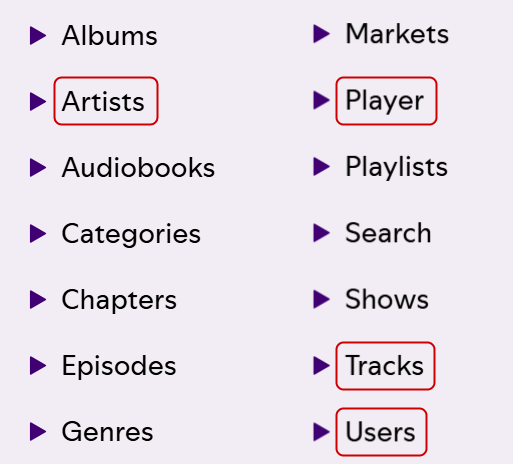
\includegraphics[width=0.4\textwidth]{figures/selected_groups.png}
    \caption{Grupos de endpoints ofrecidos y cuáles se van a usar.}
    \label{fig:selected_groups}
\end{figure}

Por razones prácticas, solo se van a mencionar los campos más relevantes en los \textit{request} y \textit{response} de los endpoints, ya que los objetos devueltos por la API suelen ser extensos y contener una gran cantidad de información, además de redundante en algunos casos. También se omite el campo de \texttt{Authorization}, que contine el \texttt{access\_token} en el \textit{header} del \textit{request}, ya que es necesario incluirlo en todas las peticiones.

\section*{Users}

En el grupo \textbf{Users} se encuentran los endpoints relacionados con la información de la cuenta del usuario. Usaremos el endpoint de \textbf{Get Current User's Profile} (figura \ref{fig:get_current_usr_profile}) para obtener datos como el nombre, correo electrónico y la imagen de perfil de la cuenta. Por otro lado, el endpoint de \textbf{Get User's Top Items} permite obtener los ``elementos'' más escuchados por el usuario, que en este caso podemos elegir entre \textit{tracks} (figura \ref{fig:get_usr_top_items_tracks}) o \textit{artists} (figura \ref{fig:get_usr_top_items_artists}).

\begin{figure}[H]
    \centering
    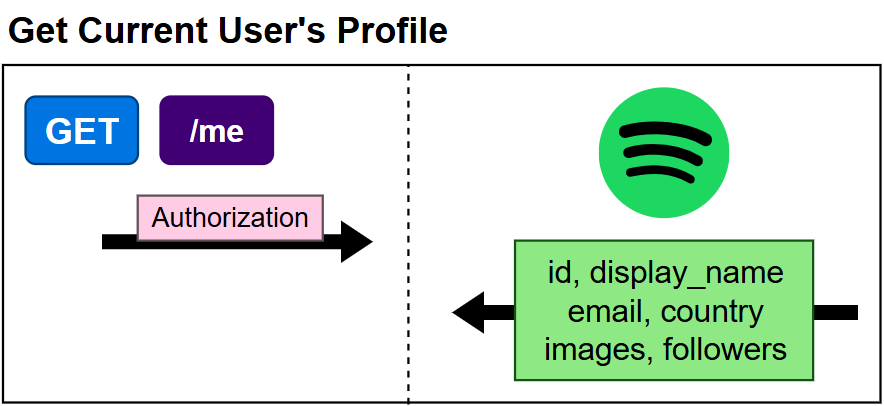
\includegraphics[width=0.75\textwidth]{figures/endpoints/get_current_users_profile.png}
    \caption{Endpoint de \textit{Get Current User's Profile}.}
    \label{fig:get_current_usr_profile}
\end{figure}

\begin{itemize}
    \item \textbf{Parámetros del Request}
          \begin{itemize}
              \item No requiere parámetros adicionales.
          \end{itemize}
    \item \textbf{Campos del Response}
          \begin{itemize}
              \item \texttt{country}: El país del usuario, en formato ISO.
              \item \texttt{display\_name}: Nombre mostrado en el perfil del usuario.
              \item \texttt{email}: Dirección de correo del usuario, ingresada al crear la cuenta.
              \item \texttt{id}: ID del usuario en Spotify.
              \item \texttt{images}: Array conteniendo las URLs de la imagen del perfil del usuarios en distintos tamaños.
              \item \texttt{followers}: Objeto con la información sobre los seguidores del usuario.
          \end{itemize}
\end{itemize}


\begin{figure}[H]
    \centering
    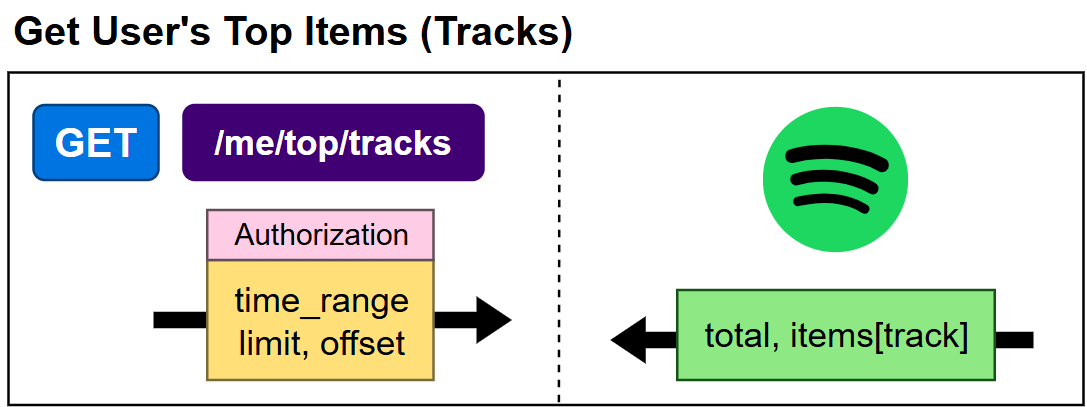
\includegraphics[width=0.75\textwidth]{figures/endpoints/get_users_top_items_tracks.png}
    \caption{Endpoint de \textit{Get User's Top Items (Tracks)}.}
    \label{fig:get_usr_top_items_tracks}
\end{figure}

\begin{itemize}
    \item \textbf{Parámetros del Request}
          \begin{itemize}
              \item \textbf{Body}
                    \begin{itemize}
                        \item \texttt{time\_range}: El marco temporal para calcular las afinidades (\texttt{"long\_term"}, \texttt{"medium\_term"} (por defecto), \texttt{"short\_term"}).
                        \item \texttt{limit}: Máximo número de elementos a devolver. Rango: 1-50.
                        \item \texttt{offset}: Índice del primer elemento a devolver.
                    \end{itemize}
          \end{itemize}
    \item \textbf{Campos del Response}
          \begin{itemize}
              \item \texttt{next}: URL de la página siguiente de elementos. \texttt{null} si no hay más elementos.
              \item \texttt{total}: Número total de elementos disponibles.
              \item \texttt{items}: Array de objetos de los datos de cada track.
                    \begin{itemize}
                        \item \texttt{name}: Nombre del track.
                        \item \texttt{popularity}: Su popularidad (0-100).
                        \item \texttt{duration\_ms}: Su duración en milisegundos.
                        \item \texttt{explicit}: Valor booleano indicando si el track contiene letras explícitas.
                        \item \texttt{album}: Información sobre el álbum donde aparece.
                              \begin{itemize}
                                  \item \texttt{id}: ID del álbum en Spotify.
                                  \item \texttt{images}: Array conteniendo las URLs de la imagen de la portada del álbum en distintos tamaños.
                                  \item \texttt{name}: Nombre del álbum.
                                  \item \texttt{release\_date}: Fecha de lanzamiento del álbum.
                              \end{itemize}
                        \item \texttt{artists}: Array con los objetos relacionados con los artistas que participaron en el track.
                              \begin{itemize}
                                  \item \texttt{name}: Nombre del artista.
                                  \item \texttt{id}: ID del artista en Spotify.
                              \end{itemize}
                    \end{itemize}
          \end{itemize}
\end{itemize}

\begin{figure}[H]
    \centering
    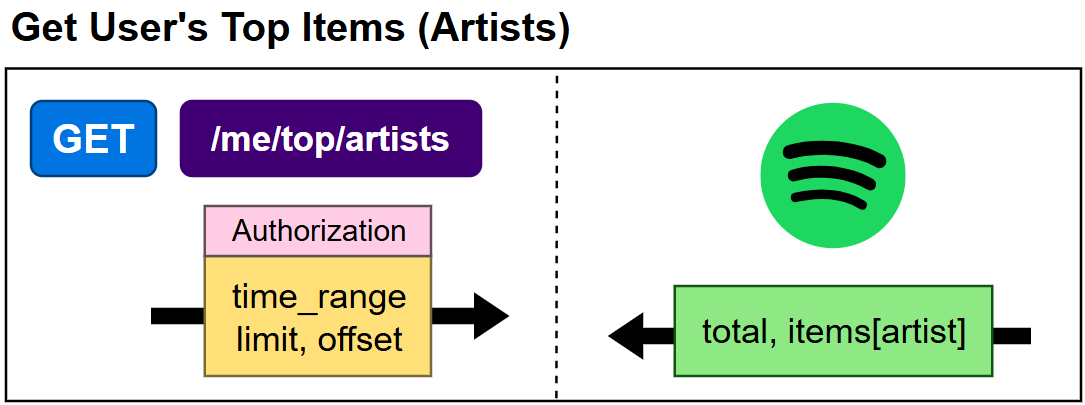
\includegraphics[width=0.75\textwidth]{figures/endpoints/get_users_top_items_artists.png}
    \caption{Endpoint de \textit{Get User's Top Items (Artists)}.}
    \label{fig:get_usr_top_items_artists}
\end{figure}

\begin{itemize}
    \item \textbf{Parámetros del Request}
          \begin{itemize}
              \item Los mismos que en el endpoint de \textit{Get User's Top Items (Tracks)}.
          \end{itemize}

    \item \textbf{Campos del Response}
          \begin{itemize}
              \item \texttt{id} (string): ID del artista en Spotify.
              \item \texttt{name}: Nombre del artista.
              \item \texttt{popularity}: Su popularidad (0-100).
              \item \texttt{followers}: Objeto con la información sobre los seguidores del artista.
              \item \texttt{genres}: Lista de géneros asociados al artista. Si el artista aún no está clasificado, el array estará vacío.
              \item \texttt{images}: Array conteniendo las URLs de la imágene del artista en distintos tamaños.
          \end{itemize}

\end{itemize}

\section*{Player}

En el grupo \textbf{Player} podemos encontrar endpoints para controlar y obtener el estado de reproducción de la cuenta. Además de poder iniciar, pausar, adelantar o controlar el volumen de la reproducción, también podemos saber las últimas canciones escuchadas por el usuario mediante el endpoint de \textbf{Get Recently Played Tracks} (figura \ref{fig:get_recently_played_tracks}).

Cabe destacar que este endpoint tiene una limitación muy considerable: \textbf{solo permite obtener las últimas 50 canciones escuchadas por el usuario}. Es decir, no es posible obtener un historial de escucha en base a un periodo de tiempo establecido, ya que esas 50 canciones pueden haber sido escuchadas en un periodo largo o en un solo día, según los hábitos de escucha del usuario. Esta limitación ha afectado en el diseño de algunas estadísticas de la aplicación, en concreto aquellas que requieren conocer los gustos musicales del usuario a lo largo del tiempo.

\begin{figure}[H]
    \centering
    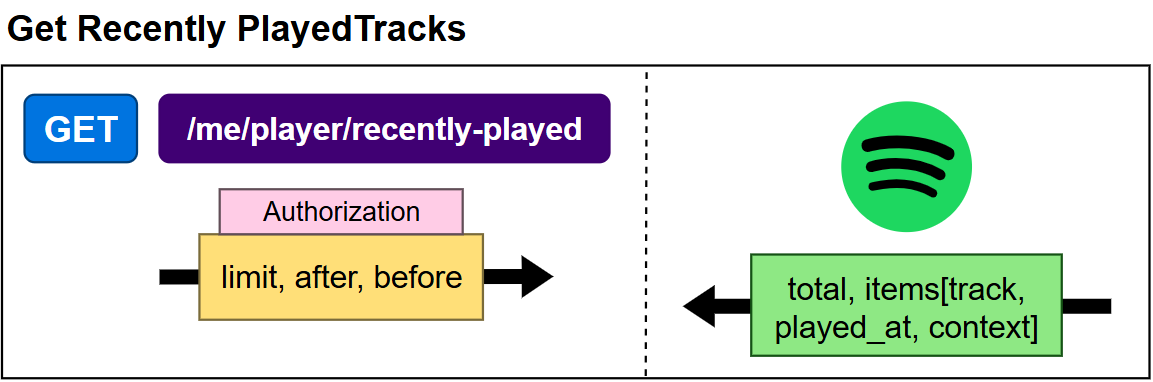
\includegraphics[width=0.85\textwidth]{figures/endpoints/get_recently_played_tracks.png}
    \caption{Endpoint de \textit{Get Recently Played Tracks}.}
    \label{fig:get_recently_played_tracks}
\end{figure}

\begin{itemize}
    \item \textbf{Parámetros del Request}
          \begin{itemize}
              \item \textbf{Body}
                    \begin{itemize}
                        \item \texttt{limit}: Número máximo de elementos a devolver. Rango: 1-50.
                        \item \texttt{after}: Marca de tiempo Unix en milisegundos. Devuelve todos los elementos posteriores (excluyendo el indicado). Si se especifica \texttt{after}, no se debe especificar \texttt{before}.
                        \item \texttt{before}: Marca de tiempo Unix en milisegundos. Devuelve todos los elementos anteriores (excluyendo el indicado). Si se especifica \texttt{before}, no se debe especificar \texttt{after}.
                    \end{itemize}
          \end{itemize}
    \item \textbf{Campos del Response}
          \begin{itemize}
              \item \texttt{next}: URL a la página siguiente de elementos. \texttt{null} si no hay más elementos.
              \item \texttt{total}: Número total de elementos disponibles.
              \item \texttt{items}: Objetos conteniendo la información sobre los tracks del historial de reproducción.
                    \begin{itemize}
                        \item \texttt{name}: Nombre del track.
                        \item \texttt{duration\_ms}: Duración en milisegundos.
                        \item \texttt{played\_at}: Fecha y hora en la que se reprodujo el track.
                        \item \texttt{explicit} (boolean): Indica si el track contiene contenido explícito.
                        \item \texttt{popularity} (integer): Popularidad del track (0-100).
                        \item \texttt{album}: Información sobre el álbum en el que se encuentra.
                              \begin{itemize}
                                  \item \texttt{name}: Nombre del álbum.
                                  \item \texttt{release\_date}: Fecha de lanzamiento.
                                  \item \texttt{images}: Las URLs de la portada del álbum en varios tamaños.
                              \end{itemize}
                        \item \texttt{artists}: Información sobre los artistas que participaron.
                              \begin{itemize}
                                  \item \texttt{name}: Nombre del artista.
                                  \item \texttt{id}: ID del artista en Spotify.
                              \end{itemize}
                    \end{itemize}
          \end{itemize}
\end{itemize}

\section*{Tracks}

Mediante los endpoints del grupo \textbf{Tracks}, se pueden obtener datos sobre canciones específicas. El endpoint \textbf{Get User's Saved Tracks} (figura \ref{fig:get_usr_saved_tracks}) devuelve las canciones guardadas en la lista de favoritos del usuario.

Este endpoint, además de permitir identificar las canciones favoritas del usuario, \textbf{proporciona una alternativa para analizar sus gustos musicales a lo largo del tiempo}. Aunque no se trata de un historial de escucha, ofrece una lista de canciones que el usuario ha decidido guardar junto con la fecha correspondiente, lo que puede servir como indicativo de sus preferencias. Esta alternativa ha sido la solución adoptada para suplir la limitación mencionada en el endpoint de \textbf{Get Recently Played Tracks}. Gracias al valor proporcionado en el campo \texttt{added\_at}, es posible considerar que el acto de añadir una canción a favoritos funciona como un proxy para representar los gustos musicales y las canciones escuchadas en torno a ese periodo de tiempo.

\begin{figure}[H]
    \centering
    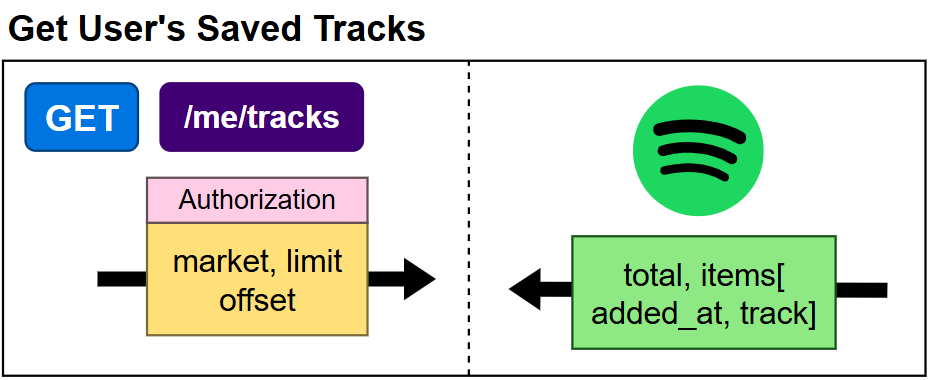
\includegraphics[width=0.75\textwidth]{figures/endpoints/get_users_saved_tracks.png}
    \caption{Endpoint de \textit{Get User's Saved Tracks}.}
    \label{fig:get_usr_saved_tracks}
\end{figure}

\begin{itemize}
    \item \textbf{Parámetros del Request}
          \begin{itemize}
              \item \textbf{Body}
                    \begin{itemize}
                        \item \texttt{market}: Código de país para indicar el mercado, en formato ISO.
                        \item \texttt{limit}: Número máximo de elementos a devolver. Rango: 1-50.
                        \item \texttt{offset}: Índice del primer elemento a devolver.
                    \end{itemize}
          \end{itemize}
    \item \textbf{Campos del Response}
          \begin{itemize}
              \item \texttt{next}: URL a la página siguiente de elementos. \texttt{null} si no hay más elementos.
              \item \texttt{total}: Número total de elementos disponibles.
              \item \texttt{items}: Array de objetos con la información del los tracks guardados.
                    \begin{itemize}
                        \item \texttt{added\_at}: Fecha y hora en la que se guardó el track en formato ISO.
                        \item \texttt{track}: Objeto con la información sobre el track.
                              \begin{itemize}
                                  \item Contiene los mismos campos que en el endpoint de \textit{Get Recently Played Tracks}.
                              \end{itemize}
                    \end{itemize}
          \end{itemize}
\end{itemize}

\section*{Artists}

Al igual que el grupo anterior, en \textbf{Artists} se pueden consultar datos sobre artistas específicos. \textbf{Get Several Artists} (figura \ref{fig:get_several_artists}) permite obtener información sobre varios artistas a la vez, reduciendo el número de peticiones realizadas a la API.

\begin{figure}[H]
    \centering
    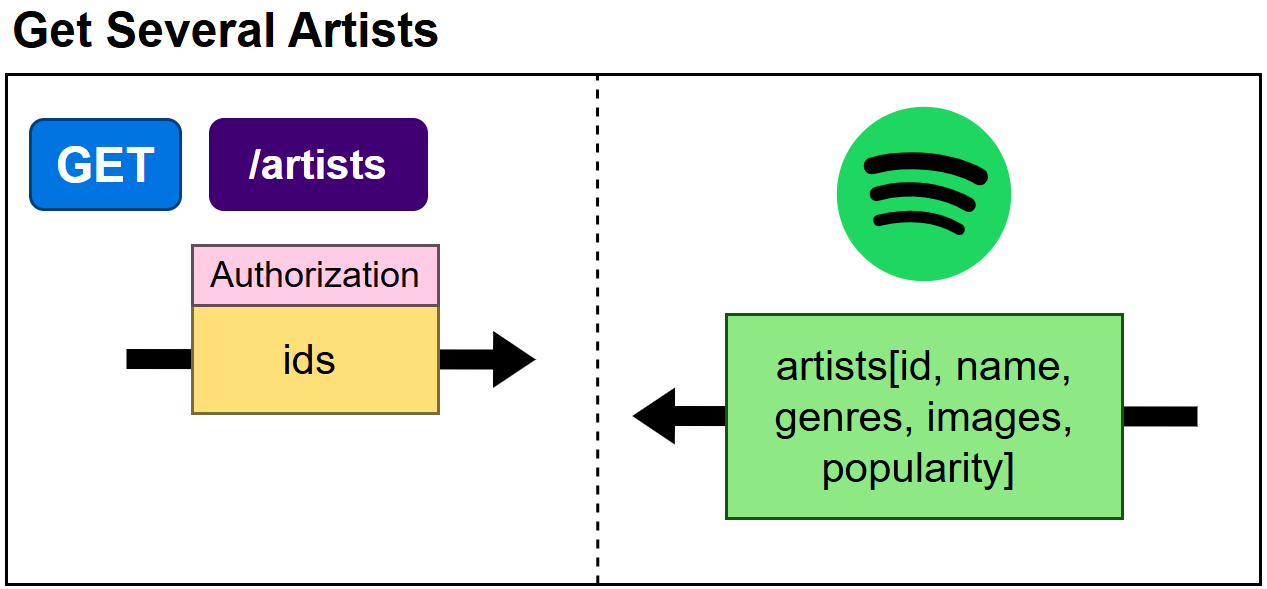
\includegraphics[width=0.75\textwidth]{figures/endpoints/get_several_artists.png}
    \caption{Endpoint de \textit{Get Several Artists}.}
    \label{fig:get_several_artists}
\end{figure}

\begin{itemize}
    \item \textbf{Parámetros del Request}
          \begin{itemize}
              \item \textbf{URL params}
                    \begin{itemize}
                        \item \texttt{ids}: Lista separada por comas de los IDs de Spotify de los artistas.
                    \end{itemize}
          \end{itemize}
    \item \textbf{Campos del Response}
          \begin{itemize}
              \item \texttt{artists}: Lista de objetos con la información de los artistas.
                    \begin{itemize}
                        \item \texttt{name}: Nombre del artista.
                        \item \texttt{id}: Su ID en Spotify.
                        \item \texttt{popularity}: Su popularidad (0-100).
                        \item \texttt{followers}: Información sobre sus seguidores.
                        \item \texttt{genres}: Lista de géneros asociados al artista.
                        \item \texttt{images}: Array de URLs de la imagen del artista en varios tamaños.
                    \end{itemize}
          \end{itemize}
\end{itemize}




% \begin{figure}[H]
%     \centering
%     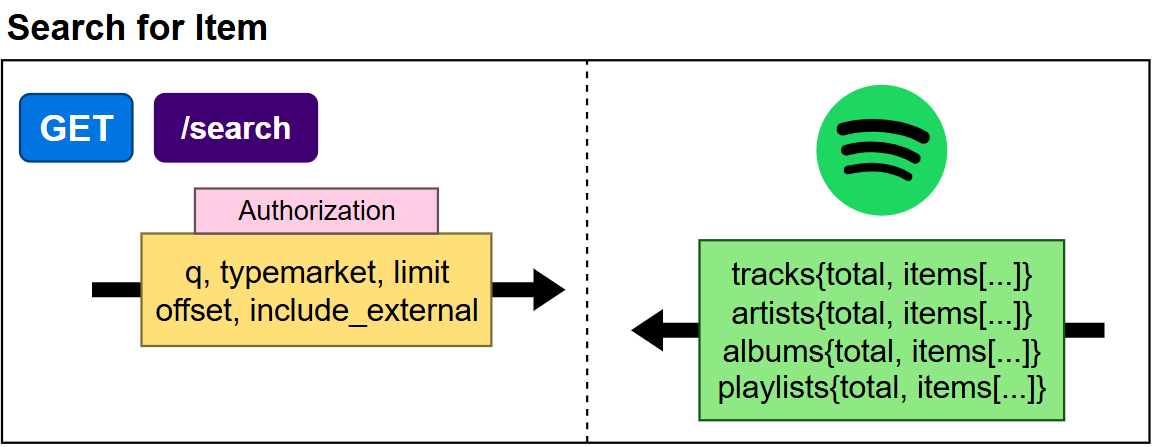
\includegraphics[width=\textwidth]{figures/endpoints/search_for_item.png}
%     \caption{Endpoint de \textit{Search for Item}.}
%     \label{fig:search_item}
% \end{figure}

% \begin{figure}[H]
%     \centering
%     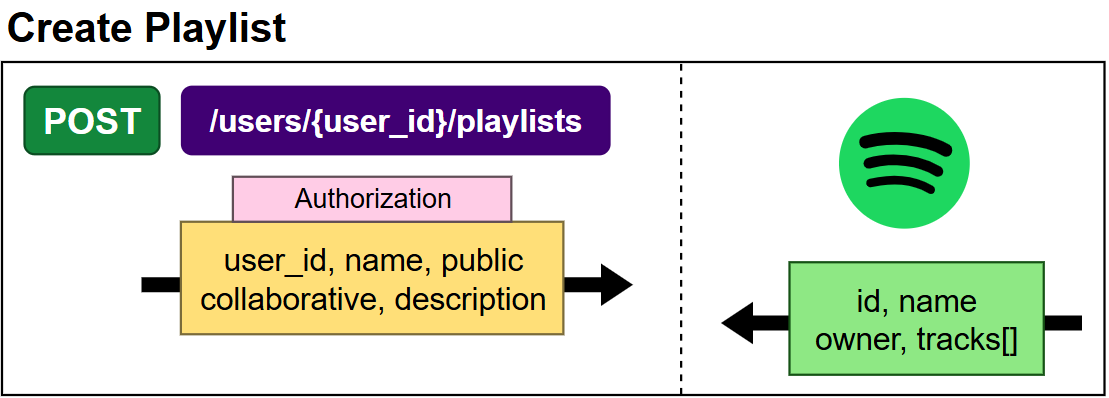
\includegraphics[width=\textwidth]{figures/endpoints/create_playlist.png}
%     \caption{Endpoint de \textit{Create Playlist}.}
%     \label{fig:create_playlist}
% \end{figure}

% \begin{figure}[H]
%     \centering
%     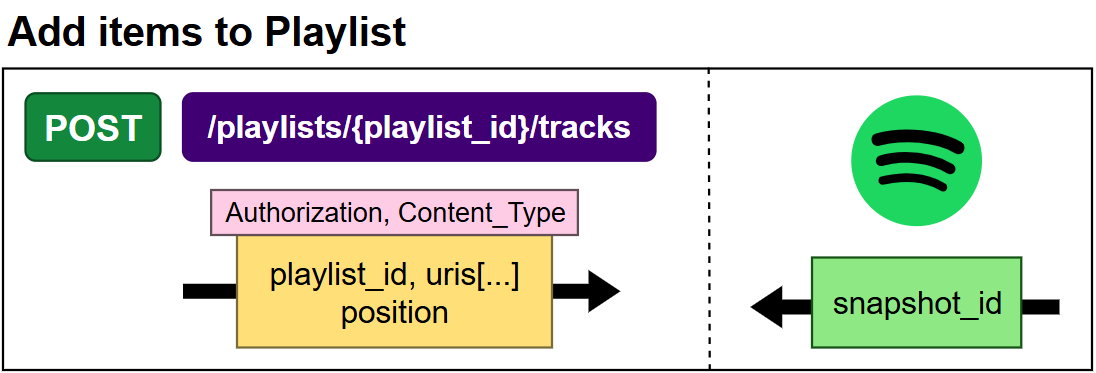
\includegraphics[width=\textwidth]{figures/endpoints/add_items_to_playlist.png}
%     \caption{Endpoint de \textit{Add Items to Playlist}.}
%     \label{fig:add_items_playlist}
% \end{figure}

% \begin{figure}[H]
%     \centering
%     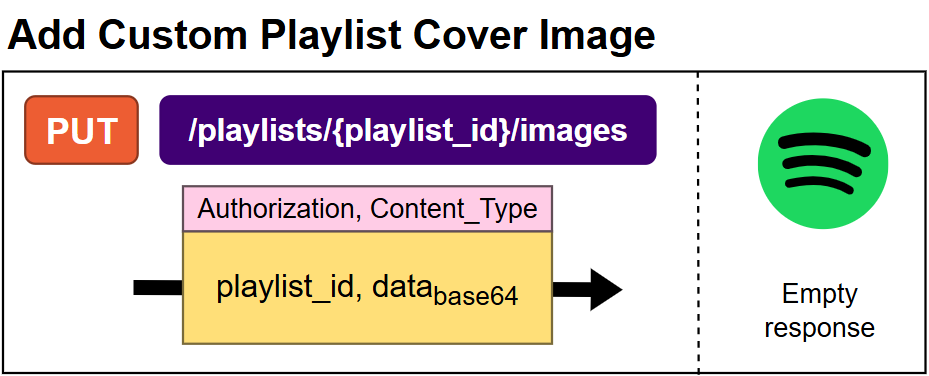
\includegraphics[width=\textwidth]{figures/endpoints/add_custom_playlist_cover_image.png}
%     \caption{Endpoint de \textit{Add Custom Playlist Cover Image}.}
%     \label{fig:add_custom_playlist_cover_img}
% \end{figure}

Los datos proporcionados por estos endpoints serán utilizados para poblar de información la aplicación, procesándolos y adaptándolos cuando sea necesario para ofrecer una experiencia personalizada al usuario. Además, estos datos influirán directamente en el diseño de la aplicación, tanto en los componentes del frontend, como en la estructura del servidor y la comunicación entre ambos.

\subsection{Scopes Necesarios}

Como ya se ha mencionado en el apartado \ref{subsubsec:scopes}, para poder tratar los datos necesarios, el usuario deber autorizar el acceso a ciertos recursos de su cuenta. Para ello, es necesario indicar los scopes adecuados al solicitar la autorización. En este proyecto, se necesitarán los siguientes scopes:

\setlength{\columnsep}{-1em} % Espacio entre columnas
\begin{multicols}{2} % Especifica que quieres dos columnas
    \begin{itemize}
        \setlength{\itemsep}{0.3em} % Espacio entre elementos
        \setlength{\topsep}{0.5em}  % Espacio al inicio de la lista
        \setlength{\parsep}{0pt}    % Espacio entre párrafos dentro de un item
        \setlength{\parskip}{0pt}   % Espacio entre párrafos
        \item \texttt{user-top-read}
        \item \texttt{user-read-private}
        \item \texttt{user-read-email}
        \item \texttt{user-read-recently-played}
        \item \texttt{user-library-read}
    \end{itemize}
\end{multicols}

\subsection{Limitaciones y Consideraciones}

Además del límite de 50 canciones en el endpoint de \textbf{Get Recently Played Tracks} y otras limitaciones relacionadas con el acceso a datos concretos, la principal limitación impuesta por la API de \textit{Spotify} es la \textbf{tasa de peticiones} o  \textit{\textbf{rate limit}}. Esta limitación se establece para evitar la sobrecarga de los servidores y garantizar un funcionamiento estable del servicio. La tasa de peticiones de Spotify se calcula en una ventana de 30 segundos (figura \ref{fig:rate_limit}). Si la aplicación supera este límite en dicho periodo, recibirá una respuesta de error \texttt{429 Too Many Requests} y los recursos solicitados quedarán temporalmente inaccesibles.

\begin{figure}[H]
    \centering
    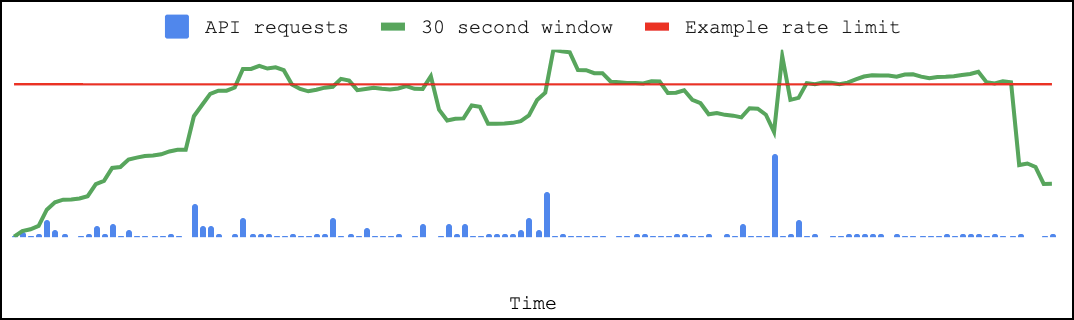
\includegraphics[width=\textwidth]{figures/rate_limit.png}
    \caption{Gráfica del funcionamiento de la tasa de peticiones, obtenida de la documentación oficial de Spotify.}
    \label{fig:rate_limit}
\end{figure}

Para evitar alcanzar este límite, se pueden implementar técnicas para optimizar el número de peticiones. Algunas de las que se implementarán en este proyecto son:

\begin{itemize}
    \item Batch APIs: Utilizar endpoints que permiten obtener lotes de datos en una sola petición, como el endpoint \textbf{Get Several Artists}.
    \item Lazy Loading: Retrasar las solicitudes de datos hasta que el usuario interactúe con un elemento específico, como al abrir una estadística.
\end{itemize}


\subsection{Política y Términos de Uso de la API}

El uso de la API de \textit{Spotify} está regulado por un marco legal detallado, compuesto por los \textit{\textbf{Spotify Developer Terms}} y la \textit{\textbf{Spotify Developer Policy}}. Estas normativas establecen las condiciones y restricciones bajo las cuales se puede acceder, procesar y utilizar los datos proporcionados por la API. A continuación, se analizan los aspectos que afectan el desarrollo del proyecto en el marco del TFG.

\subsubsection{Restricciones y Obligaciones}

Se subrayan dos principios básicos en sus términos: \textbf{la protección de los derechos de los usuarios} y \textbf{la garantía de que el contenido ofrecido en su plataforma está debidamente licenciado}. Esto implica que cualquier aplicación desarrollada debe respetar la privacidad de los usuarios y manejar los datos conforme a las preferencias que ellos definan. Además, está prohibido utilizar los datos o contenidos de \textit{Spotify} para fines no autorizados, como entrenar modelos de inteligencia artificial o crear bases de datos derivadas.

El uso de la API está sujeto a restricciones específicas, que se berán de cumplir en este proyecto. Entre las más relevantes se destacan:

\begin{itemize}
    \item \textbf{Acceso y uso de datos:} Solo se pueden solicitar los datos necesarios para operar la aplicación y deben eliminarse si un usuario decide desconectar su cuenta de \textit{Spotify}.
    \item \textbf{Prohibiciones explícitas:} Está prohibido transferir datos a terceros, crear funcionalidades que permitan \textit{stream ripping}, o desarrollar servicios destinados al uso empresarial o con contenido dirigido a menores de edad.
    \item \textbf{Caché local:} Aunque se permite el almacenamiento temporal de ciertos datos para mejorar el rendimiento, no se debe almacenar contenido indefinidamente.
    \item \textbf{Mecanismos de desconexión:} La aplicación debe ofrecer a los usuarios una forma accesible y funcional de desconectar su cuenta de \textit{Spotify} en cualquier momento.
\end{itemize}

\subsubsection{Protección de Datos y Seguridad}

Los desarrolladores son responsables de implementar medidas de seguridad estándar para proteger los datos personales de los usuarios. Esto incluye:

\begin{itemize}
    \item Proporcionar una política de privacidad clara y accesible que explique cómo se recopilan, procesan y comparten los datos.
    \item Asegurar la confidencialidad de los datos personales y notificarlos a \textit{Spotify} en caso de incidentes de seguridad que puedan comprometer esta información.
    \item Respetar las solicitudes de los usuarios relacionadas con sus datos, como la rectificación o eliminación de la información.
\end{itemize}

\subsubsection{Implicaciones para el TFG}

La implementación de la aplicación debe garantizar el cumplimiento de las políticas mencionadas, especialemente la correcta gestión de los datos personales de los usuarios y el uso correcto de los recursos. En este sentido, es importante solicitar únicamente los \textit{scopes} necesarios para las funcionalidades definidas, asegurando que cada autorización concedida por los usuarios esté justificada. También queda claro que el único uso válido del almacenamiento de los datos es el de la caché temporal en el servidor, con el propósito de optimizar el rendimiento. Además, en caso de que el usuario decida desconectar su cuenta de la aplicación, se debe implementar procesos claros y que aseguren la eliminación completa de sus datos.

\textit{Spotify} se reserva el derecho de revisar las aplicaciones que acceden a su API para garantizar que cumplan con los términos establecidos. En caso de detectar alguna infracción, como el incumplimiento de la normativa descrita, pueden limitar el acceso, revocar permisos o incluso suspender completamente la funcionalidad de la aplicación. Por lo tanto, el diseño y desarrollo de la aplicación deben incorporar estas consideraciones desde el principio, para evitar cualquier tipo de conflicto con la política de \textit{Spotify}.

% TODO: El contenido de esta sección es temporal, hay que ir mirando uno a uno cada cosa.
\section{Requisitos Funcionales}

Los requisitos funcionales describen las funcionalidades esenciales que debe cumplir la aplicación para satisfacer las necesidades del usuario. En el caso de esta aplicación, todos los requisitos funcionales están orientados al cumplimiento del objetivo principal: permitir a los usuarios acceder al análisis de sus datos musicales cuando lo deseen. Estas funcionalidades están organizadas en diferentes categorías según su ámbito.

\subsection{Autenticación y Sesión}
\begin{itemize}
    \item El usuario debe poder iniciar sesión utilizando su cuenta de \textit{Spotify} mediante OAuth 2.0.
    \item El usuario debe poder cerrar sesión desde cualquier página.
    \item El cierre de sesión debe eliminar cualquier dato asociado al usuario.
    \item La aplicación debe obtener y gestionar adecuadamente e token de acceso para interactuar con la API de \textit{Spotify}.
    \item La sesión del usuario debe permanecer activa mientras este interactúe con la aplicación web. En caso de que el tiempo de validez del token expire, el sistema debe renovar el token de forma transparente para el usuario.
\end{itemize}

\subsection{Navegación}
\begin{itemize}
    \item La aplicación debe tener una barra de navegación con acceso a las secciones:
          \begin{itemize}
              \item \textbf{Home:} Vista general de las estadísticas generales.
              \item \textbf{Stats:} Estadísticas más avanzadas y originales.
              \item \textbf{Panel de Usuario:} Panel desplegable con la opción de cerrar sesión. % y botón de ajustes
          \end{itemize}
\end{itemize}

\subsection{Estadísiticas Generales (Home)}
\begin{itemize}
    \item El usuario debe ver una página inicial con estadísticas generales relacionadas con su cuenta, siendo las siguientes:
          \begin{itemize}
              \item \textbf{Top Tracks:} Muestra los top 5 canciones del usuario.
              \item \textbf{Top Artists:} Muestra los top 5 artistas del usuario.
              \item \textbf{Top Genres:} Muestra los top 5 géneros del usuario,
              \item \textbf{Recently Played:} Muestra una lista reducida de las últimas 10 canciones escuchadas, en orden cronológico. Si el usuario quiere, podrá ver la lista completa de las 50 canciones pulsando un botón.
          \end{itemize}
    \item El usuario podrá cambiar el periodo de tiempo en el que se basan los datos de los tres tops mediante un menú desplegable.
\end{itemize}

\subsection{Estadísticas Avanzadas (Stats)}

En esta página, el usuario podrá explorar una gama de seis estadísticas más avanzadas. Cada estadística ofrece funcionalidades específicas, descritas a continuación:

\subsubsection*{Hall Of Fame}

\begin{itemize}
    \item La estadística mostrará las \textbf{top 16 canciones} del usuario en formato de cuadrícula (4x4), utilizando las portadas de los álbumes de cada canción como elemento visual.
    \item Al pasar el ratón por encima de cada una de las portadas, se mostrará el nombre de la canción y el artista.
    \item El usuario, mediante un botón, podrá crear una playlist de manera automática en su cuenta:
          \begin{itemize}
              \item Se generará una nueva playlist.
              \item Se añadirán las canciones del top 16.
              \item Se actualizará la imagen de la playlist con la representación visual de la cuadrícula de portadas generada para esta estadística.
          \end{itemize}
\end{itemize}

\subsubsection*{Huella Del Día}

% TODO: Un poco justillo la interactividad en esta estadística.
\begin{itemize}
    \item El usuario verá un gráfico de líneas, donde el eje horizontal representa las horas del día y el eje vertical los minutos de música escuchados (correspondientes a 1 hora).
    \item Al pasar el ratón por encima de un nodo de la gráfica, se mostrará la cantidad exacta de minutos escuchados en esa hora.
    \item Se indica la hora del día con más minutos de escucha.
\end{itemize}

\subsubsection*{Estaciones Musicales}

\begin{itemize}
    \item Se mostrará un gráfico en forma de anillo dividido en cuatro segmentos, cada uno representando una estación del año: invierno, primavera, verano y otoño.
    \item Al pasar el ratón por encima de un segmento del gráfico, se abrirá un panel que mostrará, basado en la actividad del usuario, el artista y el género musical destacados durante ese periodo.
    \item La información en el panel se actualiza dinámicamente mientras el usuario pasa el ratón por las distintas secciones del gráfico.
\end{itemize}

\subsubsection*{Tus Décadas}

\begin{itemize}
    \item Se presentará un histograma que muestra el número de álbumes correspondientes a cada año, agrupados por décadas. La cantidad de álbumes se muestra de manera visual, mediante imágenes de portadas apiladas en columnas. Los álbumes están asociados a las canciones favoritas del usuario, mostrando una única repetición de cada álbum, independientemente de la cantidad de canciones guardadas de ese álbum.
    \item El gráfico es explorable, permitiendo al usuario desplazarse horizontal y verticalmente.
    \item El usuario podrá hacer \textit{zoom in} y \textit{zoom out} para ajustar el nivel de detalle, permitiéndole observar las portadas de los álbumes con mayor claridad.
\end{itemize}

\subsubsection*{La Bitácora}

El usuario podrá explorar detalladamente el historial completo de sus canciones guardadas en favoritos, organizadas por fechas. Se estructura de la siguiente manera:
\begin{itemize}
    \item Se mostrará la visualización principal; un gráfico de barras con el número total de canciones guardadas, agrupadas por años, desde la creación de la cuenta hasta la fecha actual.
    \item Al hacer clic en una barra que represente un año, se profundizará en el gráfico para mostrar la distribución de canciones guardadas por meses dentro de ese año.
    \item De forma similar, al hacer clic en una barra que represente un mes, se desglosará la información para mostrar las canciones guardadas por días dentro de ese mes específico.
    \item El usuario podrá navegar libremente entre los niveles (años, meses y días), pudiendo retroceder hacia niveles superiores en cualquier momento.
    \item Al pasar el ratón por encima de cualquier barra, se mostrará el número de canciones guardadas para ese período.
    \item En el nivel de días, al pasar el ratón sobre una barra, se mostrarán además los nombres y artistas de las canciones guardadas en esa fecha específica.
\end{itemize}


\subsubsection*{Índice de Resonancia}

Se presentará al usuario, de forma visual, dos métricas relacionadas con sus preferencias musicales: la popularidad media de sus canciones guardadas en favoritos y la popularidad media de las últimas 50 canciones escuchadas. Estas métricas se implementarán a través de las siguientes funcionalidades:
\begin{itemize}
    \item Cada valor estará asociado a una onda sinusoidal animada, cuya frecuencia se ajustará proporcionalmente al valor numérico correspondiente.
    \item El usuario podrá pulsar un botón que generará una nueva onda. Esta nueva onda se calcula mediante la suma matemática de las frecuencias de las dos ondas originales, mostrando la interferencia entre las dos. Además, junto a esta nueva onda, se mostrará la diferencia numérica entre los dos valores originales.
    \item El usuario podrá pasar el ratón sobre la tarjeta de cualquiera de los valores para resaltar visualmente la onda correspondiente, facilitando la identidicación.
    \item Los cálculos y la generación de datos necesarios para esta estadística se realizarán principalmente en el servidor.
\end{itemize}

\section{Requisitos No Funcionales}

Los requisitos no funcionales de la aplicación son fundamentales para garantizar no solo su funcionalidad, sino también su rendimiento, seguridad, escalabilidad y usabilidad. A continuación, se detallan los aspectos clave que la aplicación debe cumplir para asegurar una experiencia de usuario satisfactoria y el cumplimiento de los estándares de calidad.

\subsection*{Rendimiento y Escalabilidad}

La aplicación debe ofrecer tiempos de respuesta aceptables en las operaciones críticas, como la carga inicial del \textit{Home} o la presentación de las estadísticas. El tiempo de respuesta debe ser inferior a \textbf{1 s} bajo condiciones normales de uso, con un máximo de \textbf{3 s} bajo picos de carga. Este requisito se medirá utilizando herramientas de pruebas de carga como K6, simulando hasta \textbf{50 usuarios simultáneos} realizando operaciones comunes. El objetivo es garantizar que el rendimiento del sistema satisfactorio para los usuarios, incluso en picos de carga inusuales.

\subsection*{Seguridad}

Es esencial garantizar la protección de los datos del usuario y las comunicaciones entre el frontend y el backend. Para ello, todas las conexiones deben utilizar \textbf{HTTPS}, y los tokens de acceso deben almacenarse de forma segura para prevenir ataques comunes como \textit{Cross-Site Scripting} (XSS) y \textit{Man-in-the-Middle} (MITM). Además, es necesario implementar medidas de seguridad en procesos críticos, como la autenticación de usuarios, incluyendo protección frente a ataques de tipo \textit{Cross-Site Request Forgery} (CSRF).

\subsection*{Testabilidad}

Para garantizar la calidad del sistema, se deben implementar pruebas automatizadas que cubran las funcionalidades clave de la aplicación, priorizando las partes críticas del backend y las interacciones más relevantes del frontend. Esto incluirá pruebas unitarias y de integración. La cobertura mínima objetivo será del \textbf{60\% del código}, con un enfoque en las secciones esenciales. Las pruebas se ejecutarán regularmente mediante integración continua (CI) utilizando GitHub Actions.

\subsection*{Usabilidad}

La aplicación debe ser intuitiva y fácil de usar para el público general. Todas las estadísticas y funcionalidades deben presentarse de manera clara. Este requisito se evaluará mediante pruebas de usabilidad con al menos \textbf{5 usuarios representativos}, asegurando que puedan completar tareas concretas sin dificultad ni confusión.


\section{Casos de Uso}

En esta sección se describen los principales casos de uso de la aplicación, relacionados con los requisitos funcionales mencionados. Cada caso de uso se enfoca en un objetivo específico que un usuario puede alcanzar utilizando las funcionalidades del sistema.

\subsection{Actores}

En este sistema, interactúan tres actores diferentes con la aplicación: el usuario anónimo, el usuario autenticado y la API de \textit{Spotify}. A continuación, se describen los roles de cada uno:

\begin{itemize}
    \item \textbf{Usuario Anónimo:} Este actor representa a los usuarios que no han iniciado sesión en la aplicación. Su única interacción con el sistema es el de inicio de sesión.
    \item \textbf{Usuario Autenticado:} Este actor es el usuario que ha iniciado sesión correctamente en la aplicación. Tiene acceso a todas las funcionalidades. Es considerado como el actor principal.
    \item \textbf{Web API de Spotify:} Este actor es el servicio de \textit{Spotify} que proporciona un sistema de autenticación y los datos necesarios para generar las estadísticas. Interactúa principalmente con el backend de la aplicación.
\end{itemize}


\subsection{Modelo de Casos de Uso}

En el modelo presentado en la figura XX, se destacan las funcionalidades principales de la aplicación y su relación con los actores: \textbf{Usuario Anónimo} y \textbf{Usuario Autenticado}, que interactúan directamente con el sistema, y la \textbf{API de Spotify}, que actúa como proveedor de datos.

\begin{figure}[H]
    \centering
    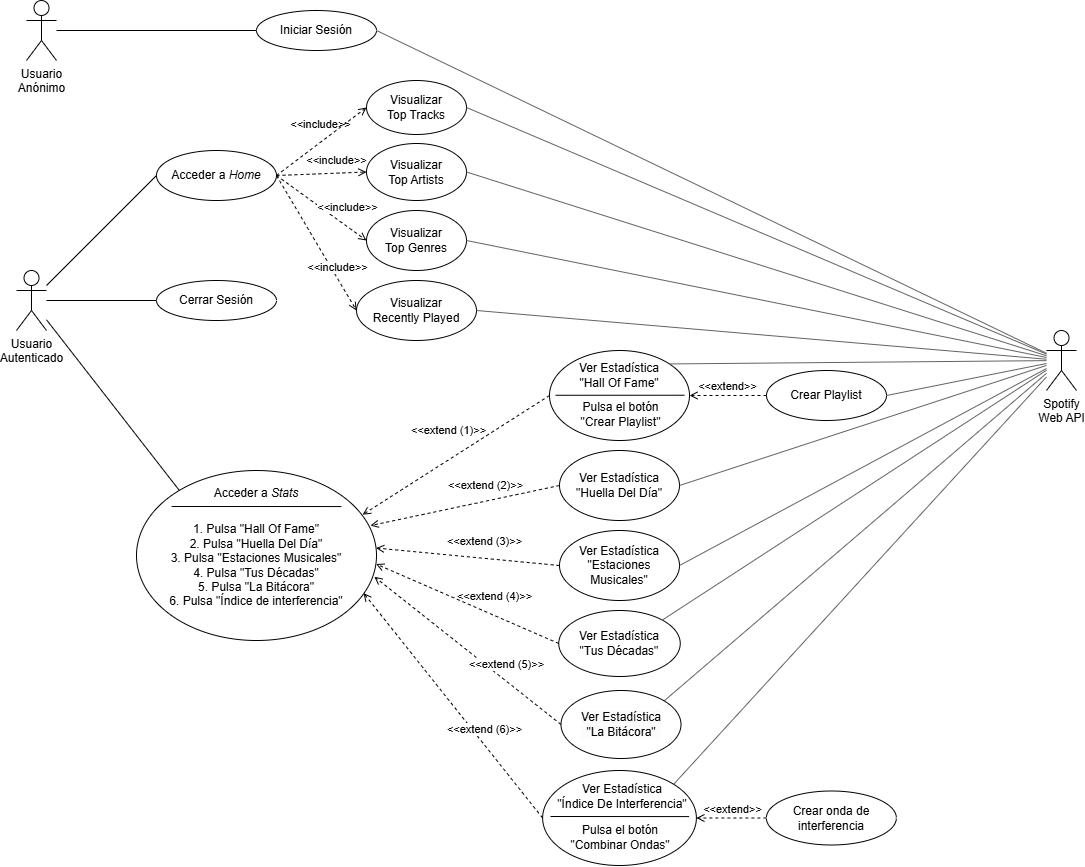
\includegraphics[width=\textwidth]{figures/modelo_casos_uso.png}
    \caption{Modelo de casos de uso del sistema.}
    \label{fig:modelo_casos_uso}
\end{figure}

% TODO: Ir describiendo el flujo de cada caso de uso.